\section[Estimation of Distribution]{分布拟合}\label{sec:2}
\subsection[Length]{长度参数}\label{sec:2-1}
\begin{frame}{长度参数}
    对于椭球的九个参数,与长度有关的三个参数${S_x, S_y, S_z}$可以看作一类。\cite{warburton1980stereological}中提到,工程实际应用中这三个参数通常来自于指数分布族(公式(\ref{equ:exp}))或者对数正态分布族(公式(\ref{equ:LogNorm}))。
    \begin{equation}\label{equ:exp}
    	% \adddotsbeforeeqnnum
    	f(x, \lambda) = \lambda\exp(-\lambda x), \quad x > 0
    \end{equation}
    
    \begin{equation}\label{equ:LogNorm}
    	% \adddotsbeforeeqnnum
    	f(x, \mu, \theta) = \frac{1}{\sqrt{2\pi}\sigma}\exp(-\frac{1}{2\sigma^2}(\ln x - \mu)^2), \quad x > 0
    \end{equation}
\end{frame}

\begin{frame}
\fs{
    	这两种分布都有可能是椭球长度的参数符合的分布,本文利用了Kolmogorov-Smirnov检验统计量在两种分布之间的选取更符合实际情况的分布。\\
   		\alert{以$S_x$为例具体流程如下:}
	\begin{itemize}
		\item 首先假设样本$S_x$符合对数正态分布函数Log-N$(\mu, \sigma^2)$。利用我们已有的样本$\{X_1, X_2, \dots, X_n\}$计算出正态分布参数的矩估计得到$\log(L_x) \sim {\rm N}(\hat{\mu}, \hat{\sigma}^2)$。进而利用\cite{page1977approximations}介绍的逼近正态分布分布函数的方法得到逼近分布函数$F_{lognormal}(x)$。
		\item 第二步假设样本$S_x$符合指数分布函数${\rm Exp}(\lambda)$,同样利用矩估计得到分布函数$F_{exponential}(x)$。
		\item 第三步根据样本$\{X_1, X_2, \dots, X_n\}$构造阶跃函数(其它的非参数方法得到的分布也可):
		\begin{equation}
			F_n(x) = \frac{1}{n}\sum_{i = 1}^{n}I_{[-\infty, x]}(X_i)
		\end{equation}
		\item 最后分别将$F_{lognormal}$和$F_{exponential}$带入公式
		\begin{equation}\label{equ:KS}
		D = \sup_x|F_n(x) - F(x)|	
		\end{equation}
		的$F(x)$中,算出两个$D$值,使得$D$值较小的分布就作为样本的分布函数,相对应的概率密度函数也就可以作为样本分布的概率密度函数。
	\end{itemize}
}
\end{frame}

\subsection[Angle]{角度参数}\label{2-2}
\begin{frame}{角度参数}
\fs{
	因为椭球可以进一步简化为扁平的椭圆,椭球的三个角度参数则转化为该椭圆的法线方向在球面坐标系(如下图)中的两个参数$(\varphi, \theta)$和椭圆在所在平面内旋转的角度$\gamma$(指的是旋转方向与X轴的夹角)。\\

为了更好地描述这三个参数,我们采用Fisher分布\footcite{fisher1953dispersion}\\

Fisher分布描述的是集中于空间或平面内某个角附近随机分布的角,由集中角度和集中程度$\kappa$两个参数决定,$\kappa$越大集中程度越高。\footnote{\fs{$(\varphi, \theta)$用三维空间Fisher分布,$\gamma$用二维平面的Fisher分布}}\\

公式(\ref{equ:fisher})是二维Fisher分布的表达式。集中角度为$\theta_0$,集中程度为$\kappa$
}


\begin{equation}\label{equ:fisher}
	%\adddotsbeforeeqnnum
	\mathrm{d}f(\theta) = \frac{\kappa}{2\sinh\kappa}\exp(\kappa\cos(\theta - \theta_0))\sin(\theta - \theta_0)\mathrm{d}\theta
\end{equation}

\begin{columns}
    \column{.3\textwidth}
    \begin{figure}[!htbp]
    	\centering
    	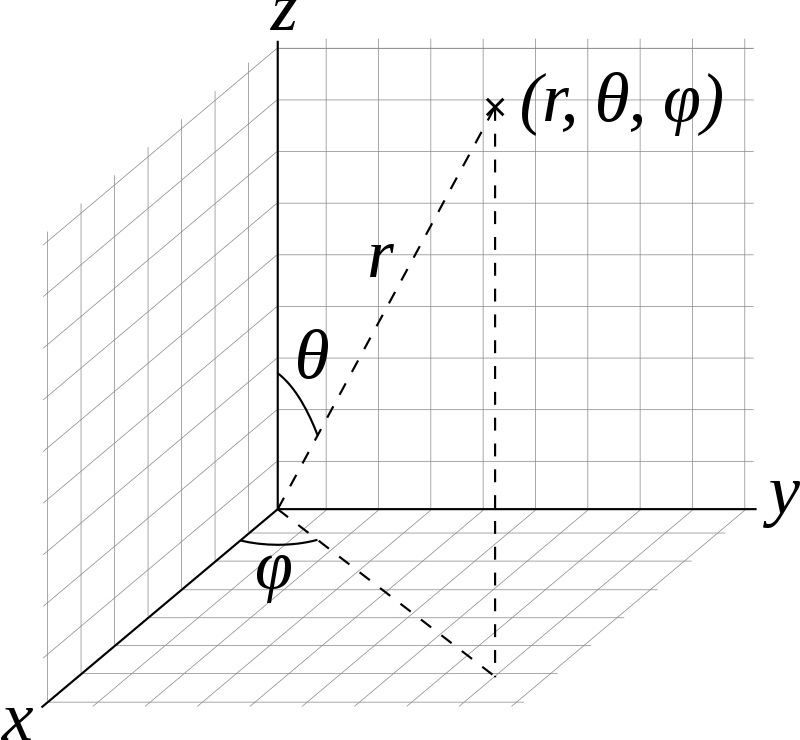
\includegraphics[width=2.5cm]{figure/Spherical}
    	\caption{球面坐标系}
    	\label{fig:Spherical}
    \end{figure}
    \column{.3\textwidth}
      \begin{figure}[!htbp]
		\centering
			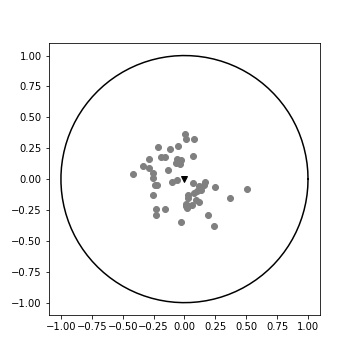
\includegraphics[width=2.5cm]{figure/fisher_k30}
			\caption{Fisher分布$\kappa = 30$}
			\label{fig:fisher_k30}
    	\end{figure}
    	
    \column{.3\textwidth}
      \begin{figure}[!htbp]
		\centering
			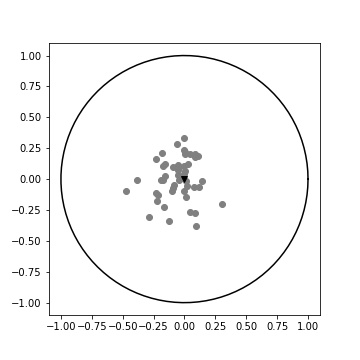
\includegraphics[width=2.5cm]{figure/fisher_k300}
			\caption{Fisher分布$\kappa = 300$}
			\label{fig:fisher_k300}
    	\end{figure}
\end{columns}
	
\end{frame}

\subsection[Location]{位置参数}\label{subsec:2-3}
\begin{frame}{位置参数}
\ff{
	与位置有关的三个参数${X, Y, Z}$没有已知的常见分布形式,但是考虑到岩体力学行为的各向同性,均匀分布可以作为一个合理的选择。另外正态分布也可以作为备选分布。接下来利用选取长度参数分布的步骤在这二者中选取合理的分布即可。

	\alert{Remark:}
	在实际工程项目中,椭圆参数的分布可能并不唯一,例如椭圆的长度参数$S_x$可能在不同的局部取样段符合不同的分布类型,在这种情况下,我们可以选取出现较多的分布类型作为全局最优的分布类型。
}
\end{frame}

\subsection[Sample]{分布拟合算例}\label{subsec:2-4}
\begin{frame}{分布拟合算例}

\ff{
	通过数值算例检验\cite{fisher1953dispersion}提到的Fisher分布参数的估计方法。

	对于二维平面的Fisher分布,考虑到二维平面角度关于原点的对称性,我们只需要对集中角度$\gamma = 0$的情况检验即可。

	分别对$\kappa = 20, 40, \dots, 300$的情况抽取$30$和$300$个样本,对这30组数据每一组重复$50$次,将拟合结果平均得出$\gamma$和$\kappa$的估计值$\hat{\gamma}$和$\hat{\kappa}$。具体拟合结果如下图

	\begin{columns}
	\column{.5\textwidth}
		\begin{figure}
		\centering
		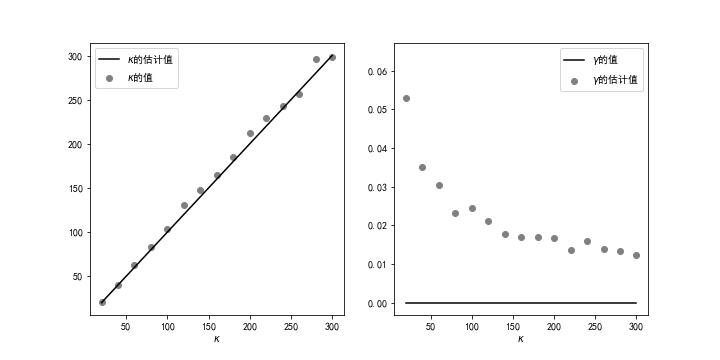
\includegraphics[width=5cm]{figure/EstFisherN30}
		\label{fig:EstFisherN30}
		\caption{Fisher分布的拟合(样本数等于30)}
		\end{figure}%
	
	\column{.5\textwidth}
		\begin{figure}
		\centering
		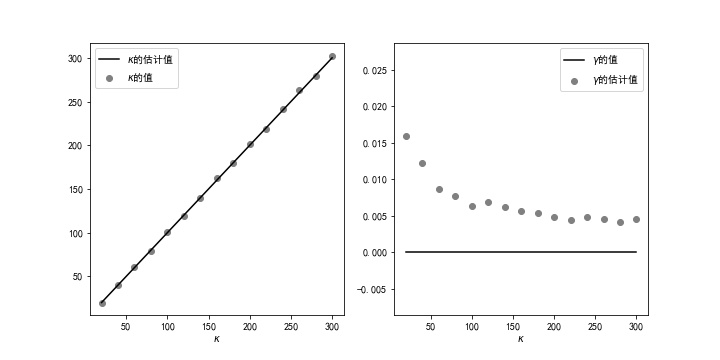
\includegraphics[width=5cm]{figure/EstFisherN300}
		\label{fig:EstFisherN300}
		\caption{Fisher分布的拟合(样本数等于300)}
		\end{figure}
	\end{columns}
}
\end{frame}